\begin{figure}[h]
\centering
\begin{minipage}[b]{0.5\linewidth}
  \centering
  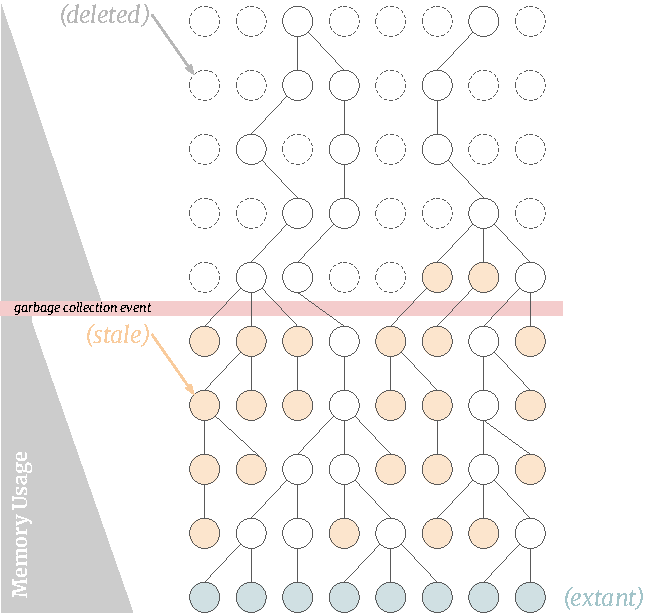
\includegraphics[width=\linewidth,height=0.3\textheight,keepaspectratio]{img/garbage-collection.pdf}
  \subcaption{garbage collection strategy}
  \label{fig:perfect-strategy:garbage-collection}
\end{minipage}%
\begin{minipage}[b]{0.5\linewidth}
  \centering
  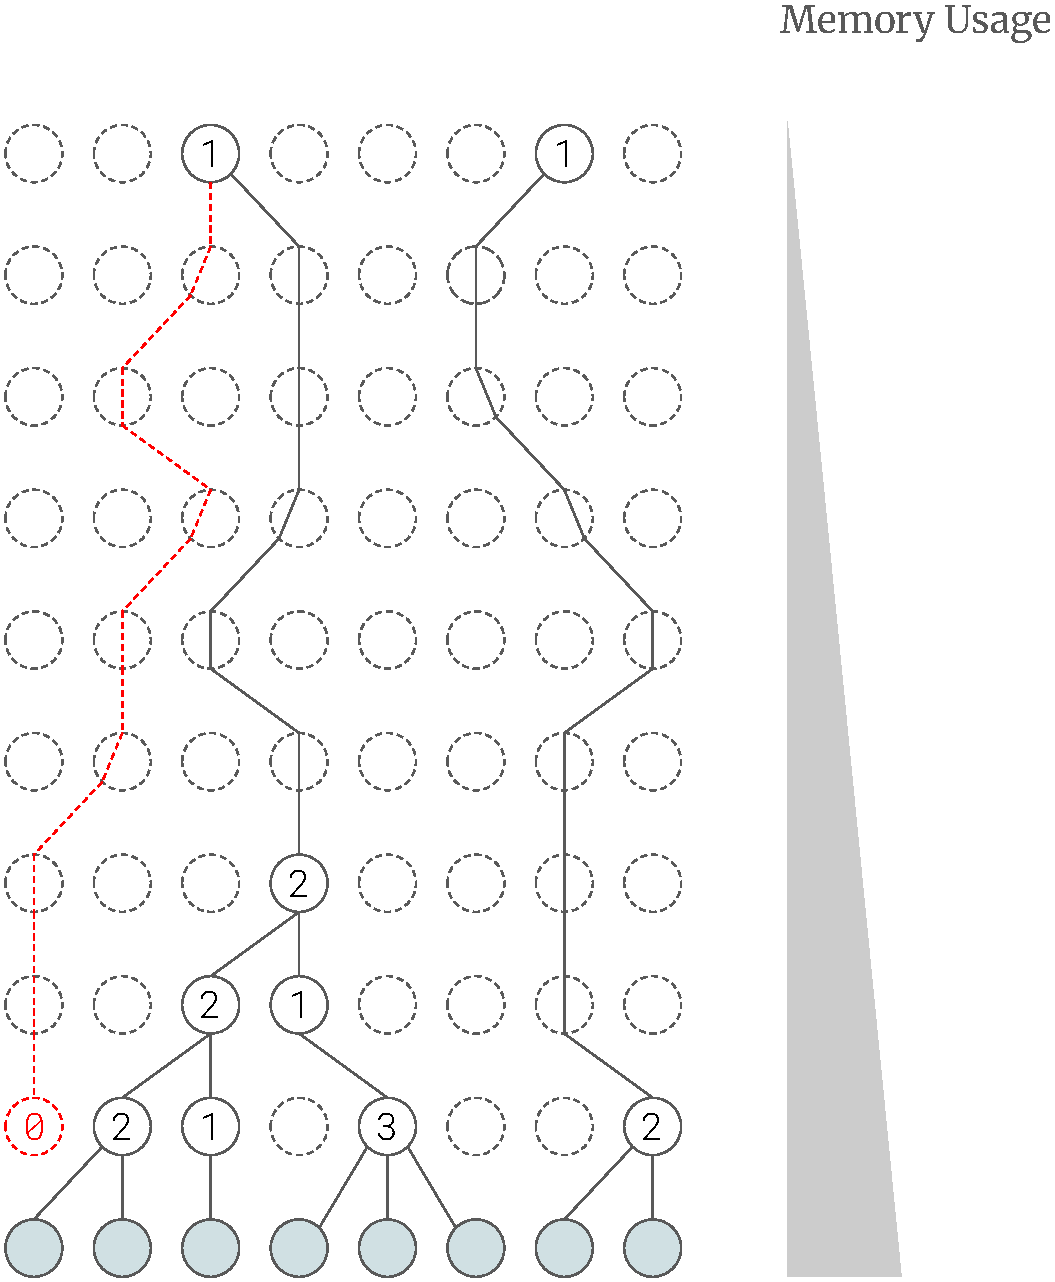
\includegraphics[width=\linewidth,height=0.3\textheight,keepaspectratio]{img/reference-counting-no-unifurcations.pdf}
  \subcaption{reference counting strategy}
  \label{fig:perfect-strategy:reference-counting}
\end{minipage}
\caption{%
\textbf{Existing state of the art versus proposed reference counting strategy.}
Under the existing garbage collection approach (panel \ref{fig:perfect-strategy:garbage-collection}), all ancestry information for all members of the current and previous populations is retained over a lookback window.
Extinct lineages are pruned during discrete garbage collection events.
Therefore, memory pressure increases substantially between garbage collection events.
By contrast, under the proposed reference counting strategy (panel \ref{fig:perfect-strategy:reference}), extinct lineages are pruned instantaneously, preventing accumulation of memory pressure between cleanup windows.
}
\label{fig:perfect-strategy}
\end{figure}
